\documentclass[11pt]{article}
\input{/Users/markwang/.preamble}
\begin{document}



\begin{enumerate}


\item \textbf{Encoder-Decoder Models and Capacity}
\begin{enumerate}
    \item The architecture will not be performant on long sequences. One reason is error signal needs to travel long distances to the encoder such that it learns the underlying structure of the language model. This introduces vanishing gradient problem during backpropagation. Another reason would be the fact that the decoder only sees the final hidden encoding $h_T^{enc}$ between encoder and decoder, each character of the input have dimishing contribution to the $h_T^{enc}$ for longer and longer sentences.
    \item Outputs 
    \begin{align*}
        seat &\rightarrow eatsay \tag{short, starts with consonant} \\
        fact &\rightarrow aftmay \\
        how &\rightarrow owhay \\
        able &\rightarrow ableway \tag{short, starts with vowel} \\
        eight &\rightarrow eitttway \\
        aches &\rightarrow amfesway \\
        shops &\rightarrow omsshay \tag{short, starts with consonant pair} \\
        shew &\rightarrow emthay \\
        shades &\rightarrow afessway \\ 
        misconstruction &\rightarrow ismosairorotesmay \tag{long, starts with consonant} \\
        prepossessing &\rightarrow epessiiensdpray \\
        reasonableness &\rightarrow efseseneeoeedway \\
        instantaneously &\rightarrow inlaaaaaa-eayylsay \tag{long, starts with vowel} \\
        insurmountable &\rightarrow insaa-icaa-eesway \\
        acknowledgments &\rightarrow amkmesinoineendway \\
    \end{align*}
    The result is usually not exactly correct. We observe that the model is able to learn to append $-ay$ to the end of words, preserve vowel characters at start of word and remove consonant characters at start of word for both short and long words. However, the model cannot remember long words as well as short words. 
\end{enumerate}

\item \textbf{Teacher-Forcing}

\begin{enumerate}
    \item During training, we utilize the actual output from the training set at current time step as inputs to the decoder in the next time step. However during testing, we do not know beforehand the groundtruth token from the previous time step to feed into the current step. There is a discrepancy between training and testing which may yield error that accumulate quickly along the generated sequence. 
    \item We can try to mitigate such discrepancy between training and testing by exposing the model, at training time, to the scenario it will experience at testing time, specifically when we feed the output of model at previous time step as input to the model at current time step. The paper proposed to, at each time step during training time, randomly pick either the groundtruth token or the token generated by the model as input to the decoder, on the account that the such sampling probability decays as training progresses to facilitate faster convergence. 
\end{enumerate}

\item \textbf{Gated Recurrent Unit (GRU)}
\item \textbf{Implementing Attention}

\newpage

\item \textbf{Attention Visualization}
\begin{enumerate}
    \item Outputs 
    \begin{align*}
        seat &\rightarrow eatsay   \tag{short, starts with 1 consonant} \\
        fact &\rightarrow actfay  \\
        how &\rightarrow owhay  \\
        drink &\rightarrow inkdray   \tag{short, starts with 2 consonant}\\
        treat &\rightarrow eattray  \\
        knees &\rightarrow eesknay  \\
        shops &\rightarrow opsshay  \\
        shew &\rightarrow ewshay  \\
        shades &\rightarrow adesshay  \\
        able &\rightarrow ableway  \tag{short + starts with vowel} \\
        eight &\rightarrow eightway  \\
        aches &\rightarrow achesway  \\
        misconstruction &\rightarrow \textcolor{red}{isconssrccteteway} \tag{long + starts with consonant} \\
        prepossessing &\rightarrow \textcolor{red}{epossesssnwpay}  \\
        reasonableness &\rightarrow \textcolor{red}{easonableneway}  \\
        instantaneously &\rightarrow \textcolor{red}{instantaaneualway}  \tag{long + starts with vowel} \\ 
        insurmountable &\rightarrow insurmountableway  \\
        acknowledgments &\rightarrow \textcolor{red}{acknowledgeenway}  \\
        aardvark &\rightarrow \textcolor{red}{aardvarkwa}  \tag{unusual/rare letter combination } \\
        marmalade &\rightarrow armalademay  \\
        apothecary &\rightarrow apothecaryway  \\
        turnpike-road &\rightarrow \textcolor{red}{urnpiksstaa-adabay} \tag{compound word with a dash } \\
        bowling-green &\rightarrow \textcolor{red}{owblnybayy-eeay}  \\
        toothpick-cases &\rightarrow \textcolor{red}{oothktcktay}  \\
    \end{align*}

    Overall, the attention-based model does a much better job at remembering words, a drawback which we noted in the non-attention-based model. The model works really well on short words (either starts with 1 consonant, consonant pairs, or vowels). The model suffers from inaccuracy for longer words and compound words with a dash, although the it is able to retain most characters from the original word, an improvement from non-attention-based model.
    

    \newpage 
    \item Success Cases \\
    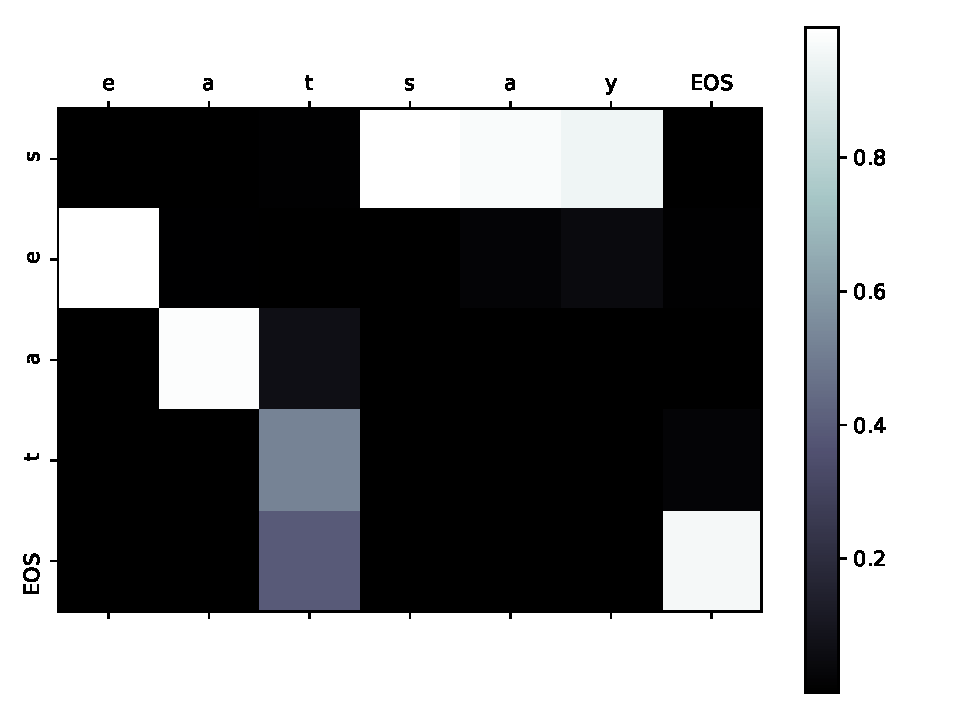
\includegraphics[width=7cm]{assets/seat.pdf}
    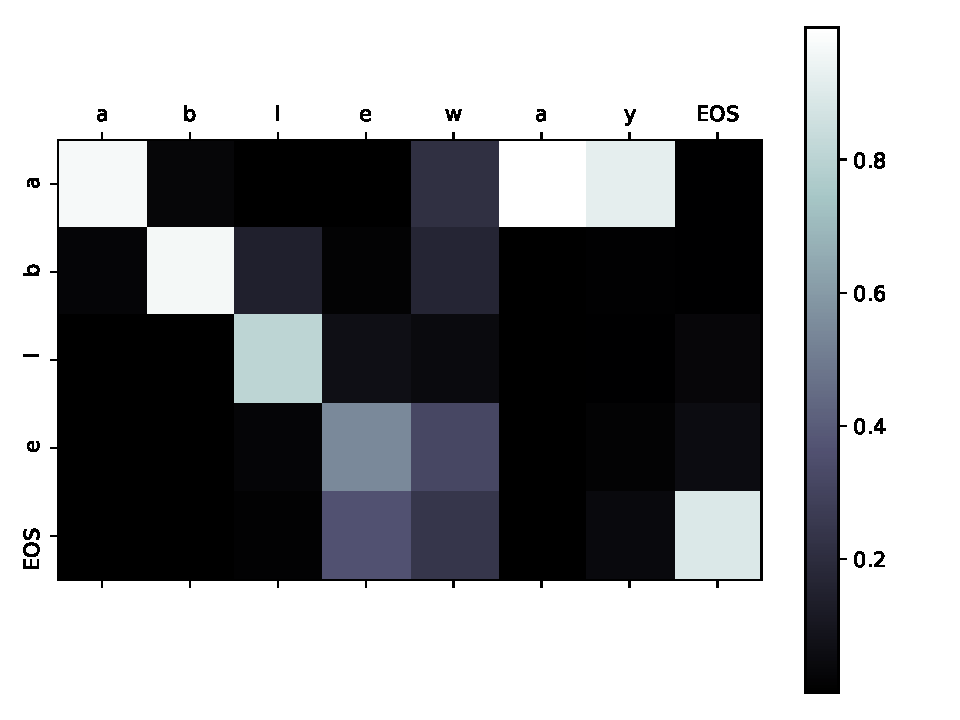
\includegraphics[width=7cm]{assets/able.pdf}
    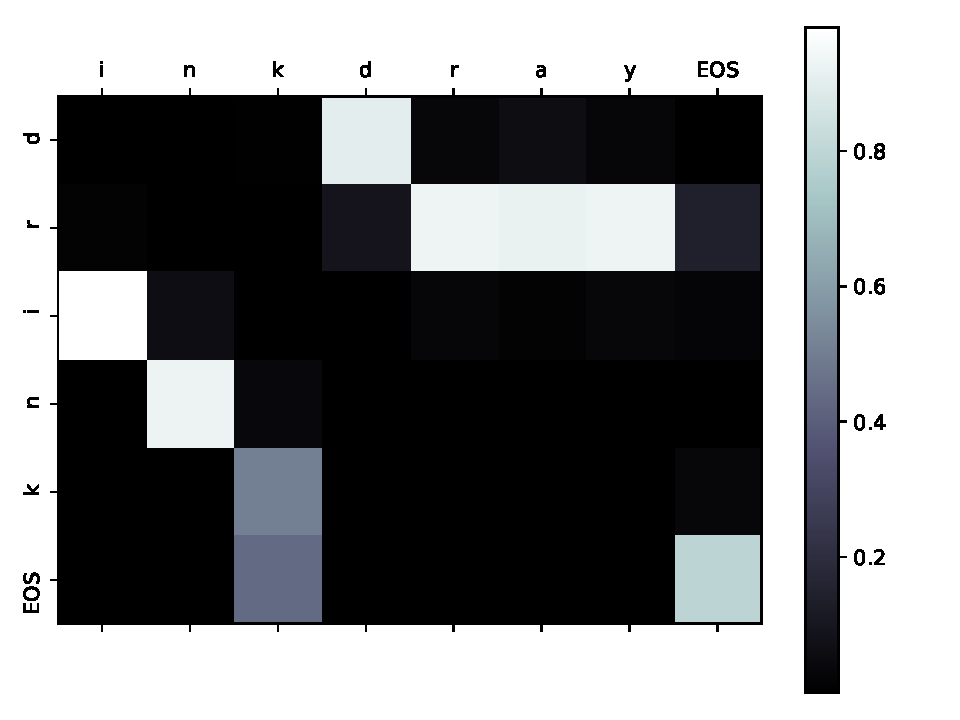
\includegraphics[width=7cm]{assets/drink.pdf}
    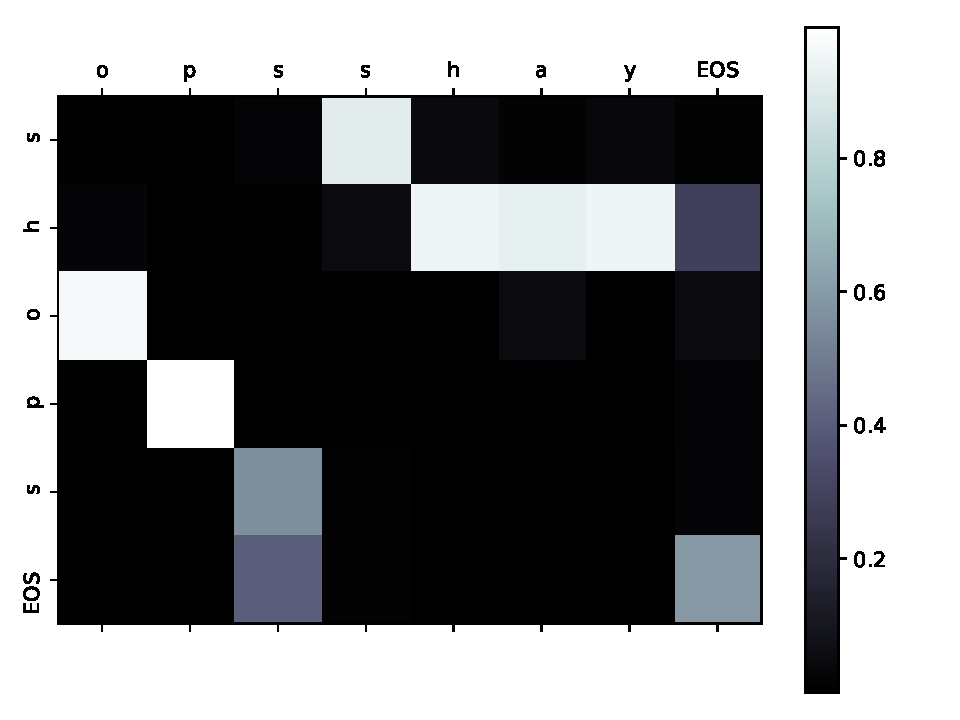
\includegraphics[width=7cm]{assets/shops.pdf}
    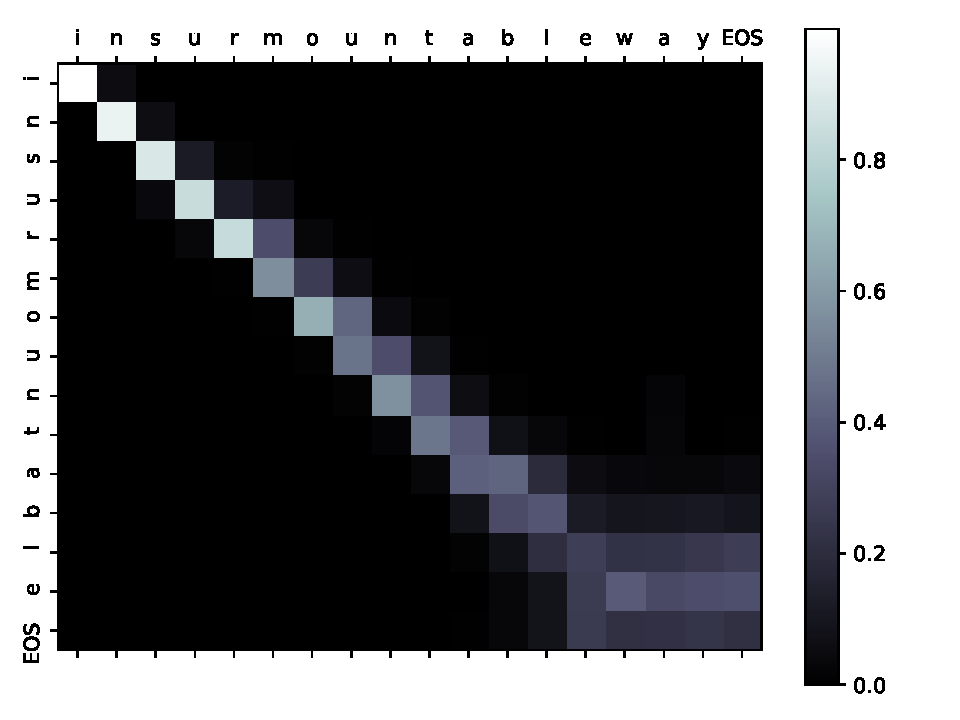
\includegraphics[width=7cm]{assets/insurmountable.pdf}
    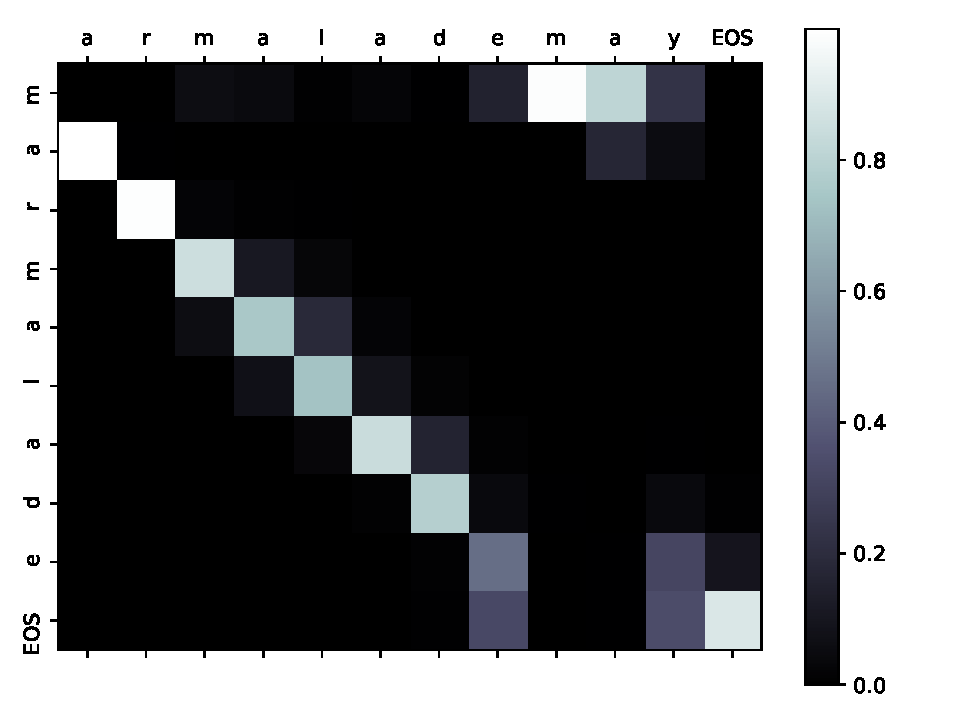
\includegraphics[width=7cm]{assets/marmalade.pdf} 
    From the attention map, we note that the model generated the correct output as it is able to pick up the patterns of the initial character(s) of the word (vowel, 1 or 2 consonants) and learns the correct identity mapping for the subsequent characters until the very end. For the last few characters, the model is able to appends the appropriate suffices for the different cases by referencing the first few characters of input word as shown in the attention map. However, we notice that $\texttt{insurmountable}$, one of the only few correctly generated long word, does not refer back to the inital characters when generating the last few characters. 
    \newpage
    \item Failure Cases \\
    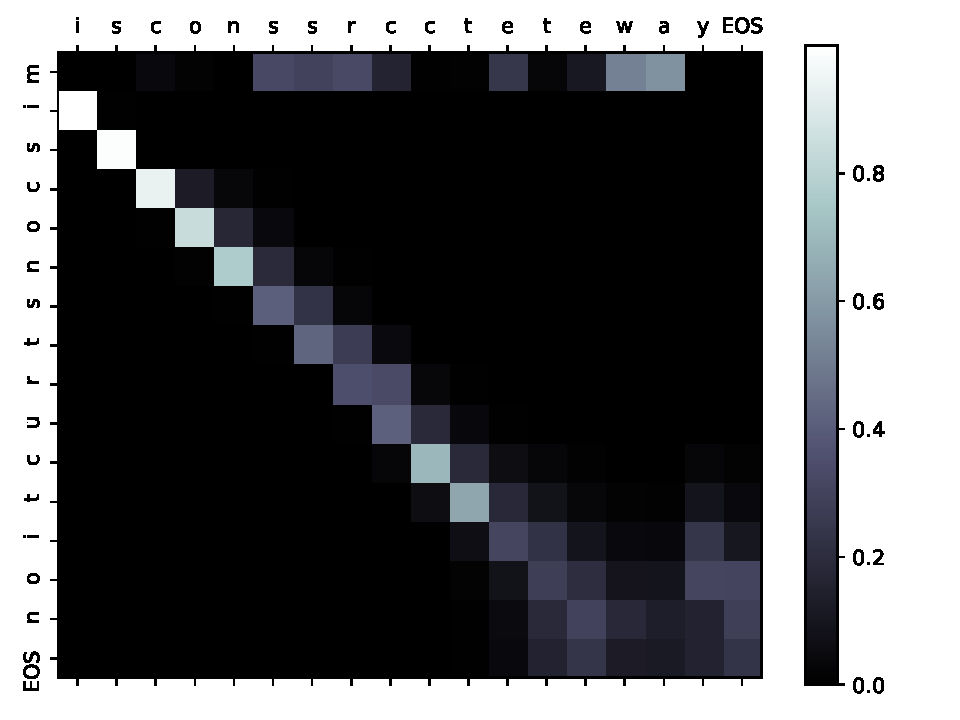
\includegraphics[width=7cm]{assets/misconstruction.pdf}
    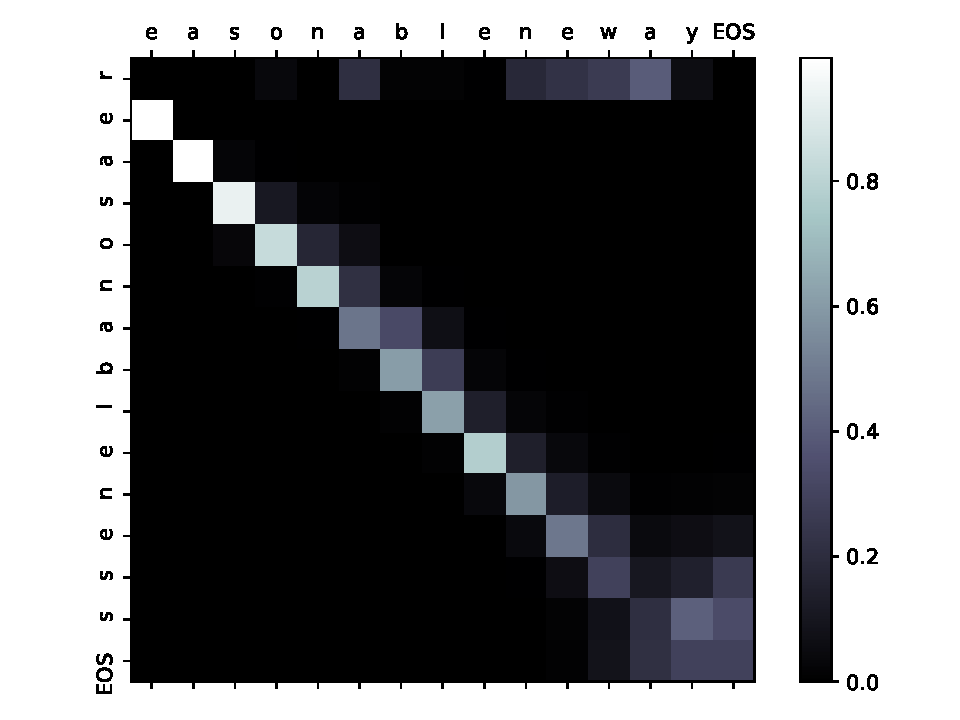
\includegraphics[width=7cm]{assets/reasonableness.pdf}
    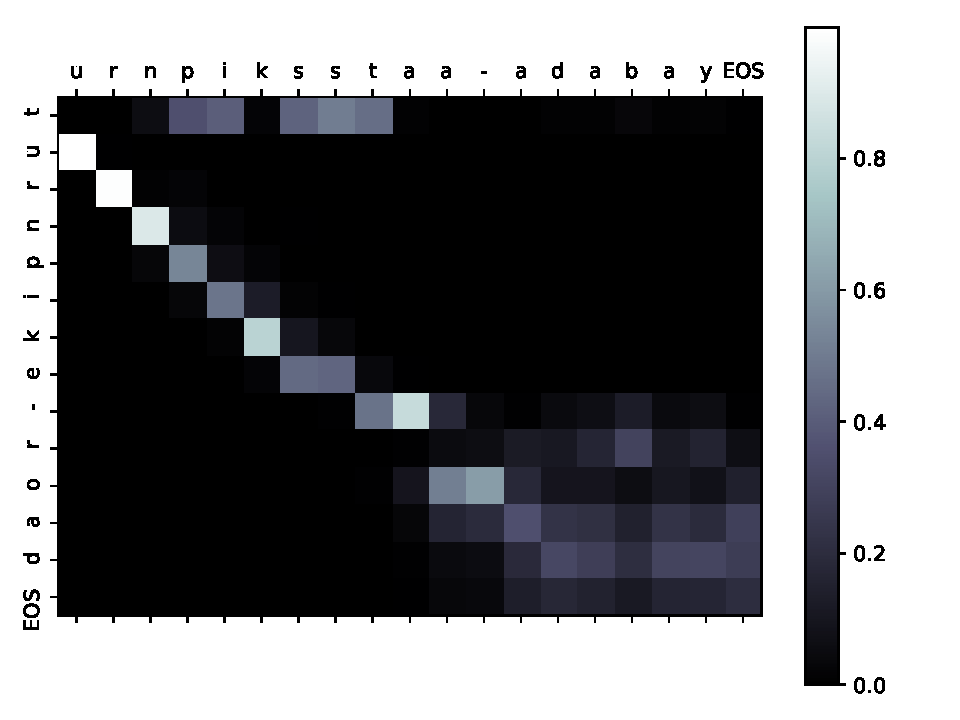
\includegraphics[width=7cm]{assets/turnpike-road.pdf}
    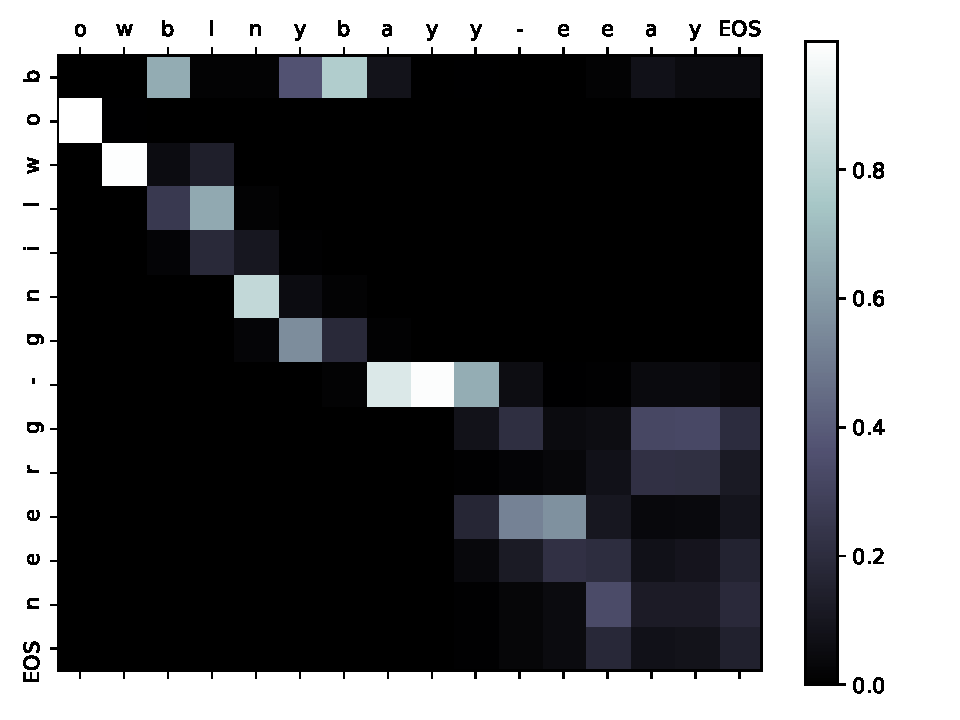
\includegraphics[width=7cm]{assets/bowling-green.pdf}
    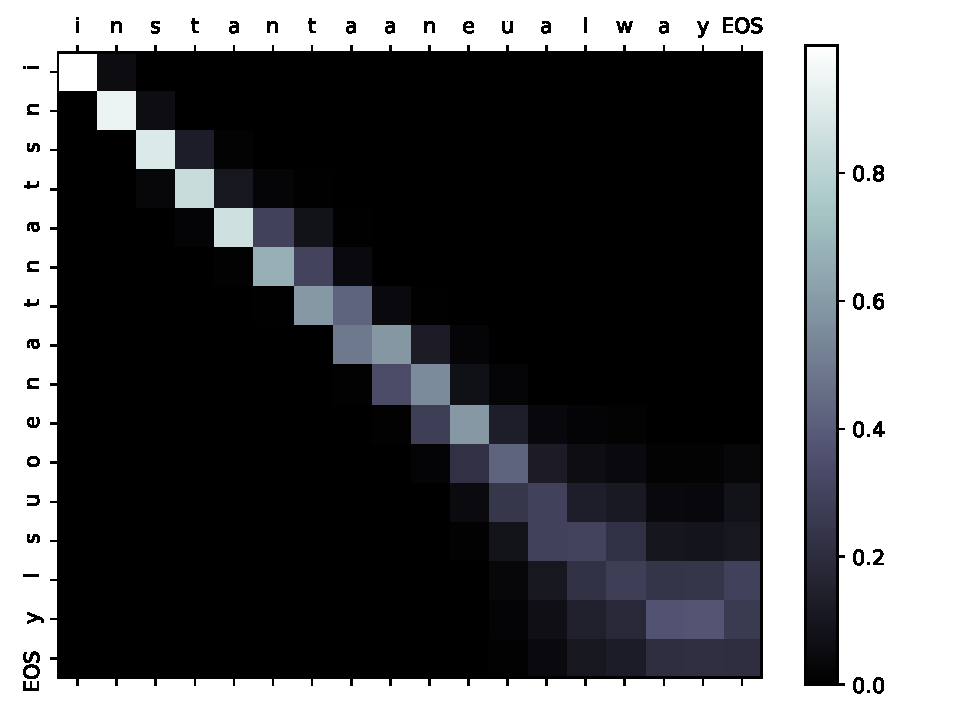
\includegraphics[width=7cm]{assets/instantaneously.pdf}
    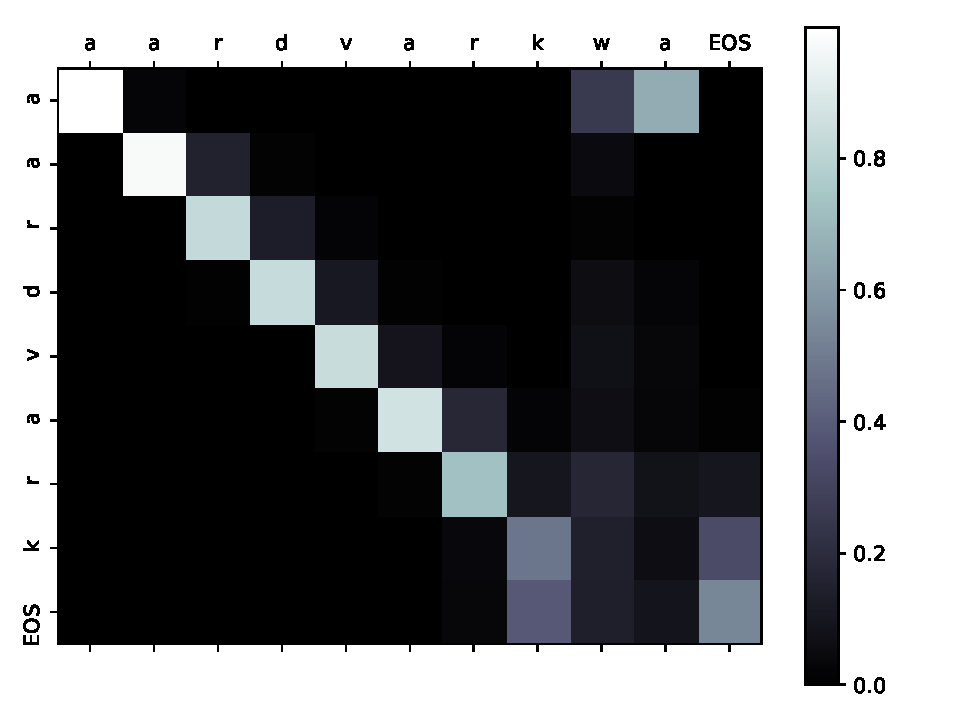
\includegraphics[width=7cm]{assets/aardvark.pdf}
    
    \begin{enumerate}
        \item One failure case is when the model prematurely references the initial characters of the input words. We observe that the model often outputs the incorrect character when the attention map for the initial characters and the characters on the diagonals are equally activated, in case of $\texttt{misconstruction}$, $\texttt{reasonableness}$, and $\texttt{turnpike-road}$. This might be because of the tendency of model to generate shorter words, as a result of the idiosyncracy of the training dataset.
        \item Another failure case arises when the input word is long enough such that the model is ambivalent about where in the input word to reference. Take $\texttt{instantaneously}$ as an example, for latter characters output from the decoder, the attention is focused on several nearby characters, centered along the diagonals. At one point, the letter $\texttt{a}$ is output twice because of such ambivalence. The failure is probably a result of the limitation of the model architecture, as it allows errors to accumulate quickly as the decoder generates the output characters. 
    \end{enumerate}

\end{enumerate}


    
\end{enumerate}










\end{document}
